\documentclass[11pt,letterpaper]{article}
\usepackage[margin=.84in,top=.78in,bottom=.79in]{geometry}
\usepackage{amsmath,amssymb,booktabs,graphicx,xcolor,hyperref,fancyhdr}
\definecolor{ink}{HTML}{19344C}\definecolor{blue}{HTML}{255795}
\hypersetup{colorlinks=true,urlcolor=blue,linkcolor=blue,pdftitle={Adaptive Gaussian Reconstruction for IDEC},pdfauthor={John Zhang and Ryan Jian}}
\pagestyle{fancy}\fancyhf{}\lhead{\small\sffamily COSI 126A \quad Unsupervised Learning and Data Mining}
\rhead{\small\sffamily Zhang and Jian}\cfoot{\small\thepage}
\setlength{\headheight}{14pt}\setlength{\parindent}{0pt}\setlength{\parskip}{5pt}
\newcommand{\sect}[1]{\vspace{3pt}{\sffamily\large\bfseries\color{ink}#1}\par}
\newcommand{\capn}[1]{{\small\color{ink}#1}\par}
\begin{document}
{\sffamily\bfseries\color{ink}\fontsize{24}{28}\selectfont Adaptive Gaussian reconstruction for IDEC}\par
{\large Weighting digit reconstruction with an image-specific center and cluster saliency}\par
{\sffamily John Zhang and Ryan Jian}\par\medskip
\textbf{Abstract.} Improved Deep Embedded Clustering (IDEC) uses reconstruction to preserve structure while learning clusters. The same objective rewards a decoder for copying details unrelated to digit identity. We reproduce the paper's MNIST accuracy to within 0.04 percentage points, then add two marks that leave every digit stroke intact. On identical marked inputs, changing the reconstruction target to the known clean digit improves clustering by 6.04 points. Our method weights pretraining errors with an image-specific circular Gaussian modulated by cluster saliency. After clean-only training, marked accuracy rises from 64.62\% with ordinary IDEC to 71.59\%. A fixed Gaussian with the same saliency reaches 71.51\%. In a separate marked-training experiment, brightening the same symbols changes fewer cluster assignments, even though a linear readout can still distinguish the brighter image from its matched partner.

\sect{1 \quad Introduction and research question}
Two handwritten sevens can differ in stroke width and still belong together. A triangle beside either seven also changes its pixels while leaving its identity intact. Both differences count toward a decoder's reconstruction error. \textbf{Our research question.} We study how the reward for reconstructing irrelevant background affects digit clustering and how much an image-specific spatial weighting can reduce its cost.

\sect{2 \quad The original method and its reproduction}
\textbf{Original research question.} Guo et al.\ investigate the effect of preserving local data structure during joint embedding and cluster learning on unsupervised clustering performance [1]. \textbf{Challenge.} DEC sharpens assignments produced by its own encoder [2]. Incorrect early assignments can distort its embedding. \textbf{Philosophy.} An embedding that still encodes enough of the input to reconstruct it should retain useful structure as clusters move. \textbf{Solution.} IDEC pretrains an autoencoder, initializes centers by K-means, and keeps the decoder during joint training. It minimizes $L_{\rm pixel}+\gamma\,\mathrm{KL}(P\Vert Q)$, where $Q$ holds Student-$t$ assignments and $P$ is their sharpened, cluster-frequency-adjusted target.

\begin{center}\small
\begin{tabular}{lrrrr}\toprule
&\multicolumn{2}{c}{Autoencoder + K-means}&\multicolumn{2}{c}{IDEC}\\
\cmidrule(lr){2-3}\cmidrule(lr){4-5} & ACC (\%) & NMI & ACC (\%) & NMI\\\midrule
Guo et al., Table 2 &81.82 &.7473 &88.06 &.8672\\
Our reproduction, seed 0 &81.85 &.7474 &88.10 &.8650\\\bottomrule
\end{tabular}\end{center}
\capn{\textbf{Table 1.} Paper reproduction using all 70,000 MNIST images for fitting and scoring. NMI measures normalized mutual information with digit identity.}
We loaded the authors' pretrained weights [3], checked their conversion against NumPy, and reached the 20,000-update limit with 0.51\% of assignments still changing. The 73.23\% ordinary IDEC control in our extension starts from fresh weights on 12,000 images and is scored on 10,000 held-out digits.

\textbf{Full-data test of our modification.} We also pretrained two fresh students from identical random weights at seed 0 on all 70,000 clean images. After 20,000 IDEC updates, ordinary IDEC reached 87.68\% ACC (NMI .8585) and our adaptive weighting reached 87.36\% (NMI .8486). The $-0.32$-point difference is one transductive run.

\newpage
\sect{3 \quad Identified limitation and hypothesis}
\textbf{Drawback.} Under uniform pixel loss, reducing squared error by one unit on a background symbol earns the same reward as doing so on a stroke. A finite-dimensional code can therefore retain irrelevant detail at a cost to digit separation. We used two tests to distinguish sensitivity to visually harder inputs from an effect of the reconstruction target itself.

\begin{center}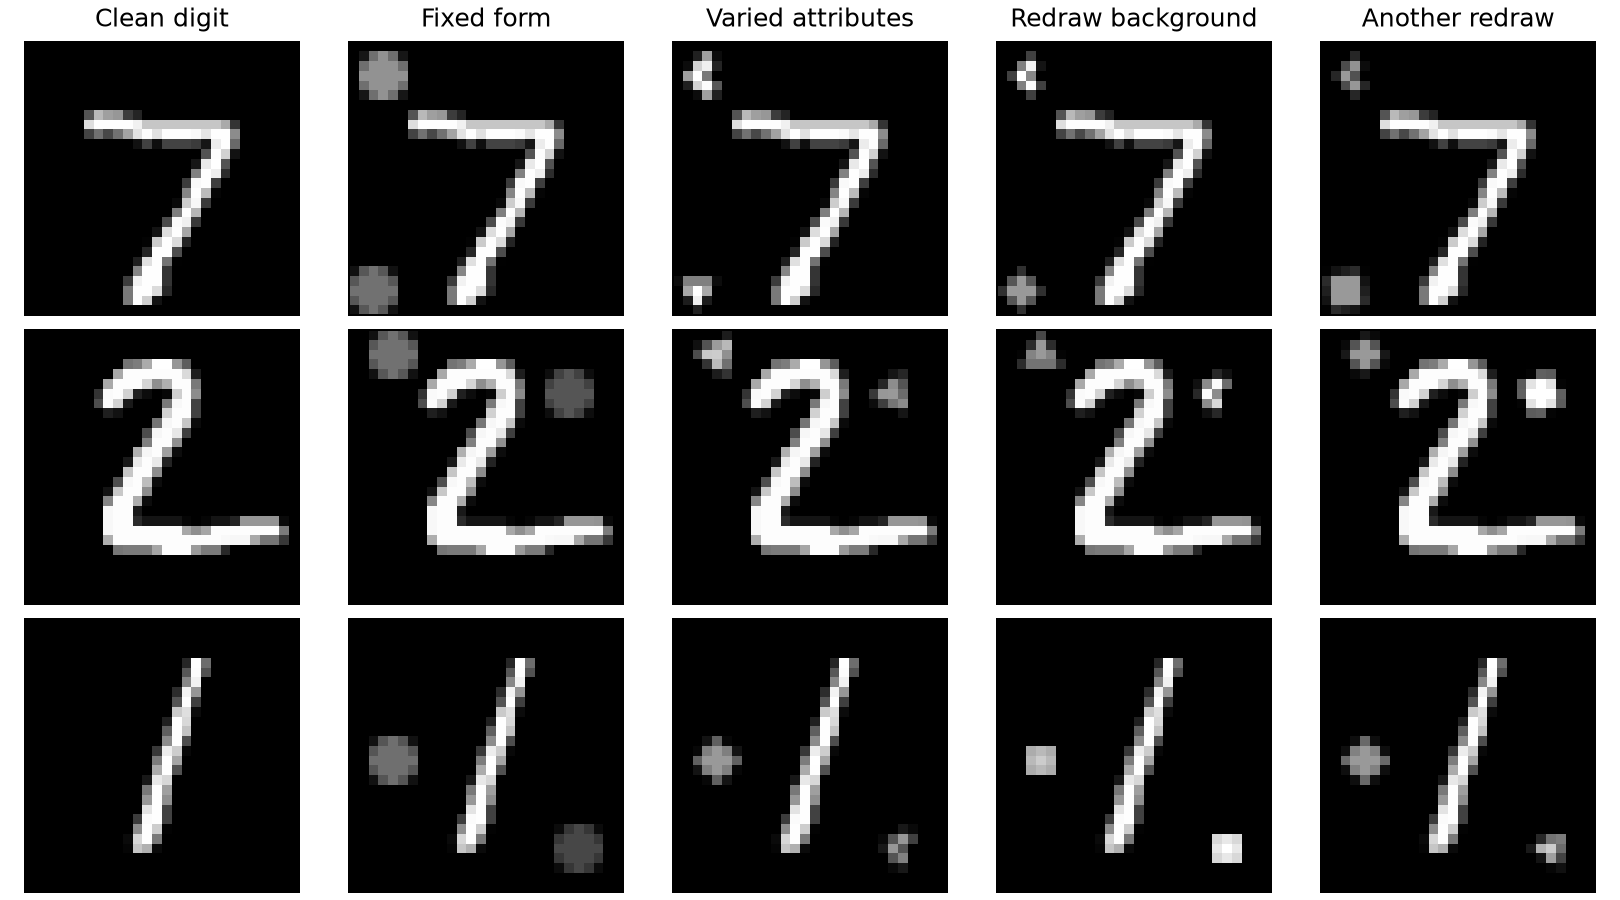
\includegraphics[width=.54\linewidth]{../figures/varied.png}\end{center}
\capn{\textbf{Figure 1.} Each row follows one digit. The generator adds two detached symbols in empty $5\times5$ boxes with a one-pixel clearance around ink. The rightmost views vary attributes at the same sites. Digits and symbols share the same grayscale channel.}

\textbf{Test 1. Do the symbols hurt both methods?} We trained and tested DEC and IDEC on clean digits, then repeated on marked versions. Within each training domain, DEC and IDEC started with the same pretrained encoder and centers. DEC fell from 77.63\% to 70.86\% ($-6.77$ points) and IDEC from 73.23\% to 65.14\% ($-8.09$). Both declined in all five seeds. IDEC's excess decline averaged 1.32 points (paired SD 3.35), positive in four seeds. Background interference also affects DEC, which drops the decoder during fine-tuning.

\textbf{Test 2. What happens when the decoder loses the reward for copying symbols?} In a separate five-seed experiment, we held the marked inputs, symbol positions and digits fixed and changed the reconstruction target. The generator supplied the original digit as a privileged diagnostic. A decoder response of one would mean the reconstructed change fully tracks the change in the input symbols.
\begin{center}\small\begin{tabular}{llrrr}
\toprule
Pretrain target & Fine-tune target & Marked ACC & Redraw flips & Decoder response\\
\midrule
Full & Full & 65.40 & 2.98 & 0.00828\\
Full & Clean & 66.85 & 2.65 & 0.00159\\
Clean & Full & 70.62 & 2.51 & 0.00289\\
Clean & Clean & 71.44 & 2.35 & 0.00145\\
\bottomrule
\end{tabular}
\end{center}
\capn{\textbf{Table 2.} On identical marked inputs, \emph{Full} targets include symbols and \emph{Clean} targets omit them. ACC and redraw flips are percentages. A flip is a cluster change when symbol attributes change.}
Using clean targets in both stages raised ACC by $6.04\pm4.37$ points (all five seeds). The decoder tracked less of the change in symbols. Changing the pretraining target alone gave most of the accuracy gain. These results implicate the reward for reproducing background, although the code may still carry background information.

\textbf{Philosophy and hypothesis.} Give more reconstruction weight to likely digit features and less to likely background. On centered digits, location gives one clue to relevance. Within that region, sensitivity of a teacher's cluster assignments gives a second clue. We predict that combining them during pretraining will improve performance when new background symbols appear at test time.

\newpage
\sect{4 \quad Adaptive Gaussian reconstruction}
\textbf{Estimate a center from each observed image.} Let $p$ be a pixel coordinate, $c_0=(13.5,13.5)$ and $G(p;c)=\exp[-\|p-c\|^2/(2\sigma^2)]$, with $\sigma=7$ pixels on $28\times28$ images. We reuse the width from the fixed prior. The intensity centroid under this prior is
\[
 c_x=\frac{\sum_p p\,x_p\,G(p;c_0)}{\sum_p x_p\,G(p;c_0)} .
\]
A blank input uses $c_0$. The center parameter specifies where reconstruction errors receive greater weight. Each image and its reconstruction target stay on the original pixel grid. The estimate uses every observed pixel and requires no digit mask.

\textbf{Estimate cluster saliency.} A frozen teacher consists of an ordinary autoencoder trained on the same unlabeled fitting images and K-means centers on its codes. For an image $x$, let $m(x)=d_2^2-d_1^2$ be the squared-distance gap between its second-nearest and nearest centers. Pixels that strongly affect this gap can help distinguish these two candidate clusters. Smooth $|x\odot\nabla_xm(x)|$ with a $3\times3$ average filter to get $a$. Set $S_x(p)=a_p/(a_p+\bar a)$, using zero for a zero signal. We cache $S_x$ in eight bits.

\textbf{Weight only student pretraining.} Normalize each image's weights to mean one, so the objective changes which errors matter while keeping their average coefficient fixed.
\[
 u_x(p)=G(p;c_x)\,[0.5+S_x(p)],\quad
 w_x(p)=u_x(p)/\overline{u_x},\quad
 L_{\rm pre}=\frac1{784}\sum_p w_x(p)(x_p-\hat x_p)^2 .
\]
After pretraining, run K-means and fine-tune with ordinary IDEC's uniform pixel MSE and $\gamma=0.1$. At inference, the student encoder and cluster centers suffice. Each training domain requires one extra teacher fit and one saliency pass, shared across student seeds.

\begin{center}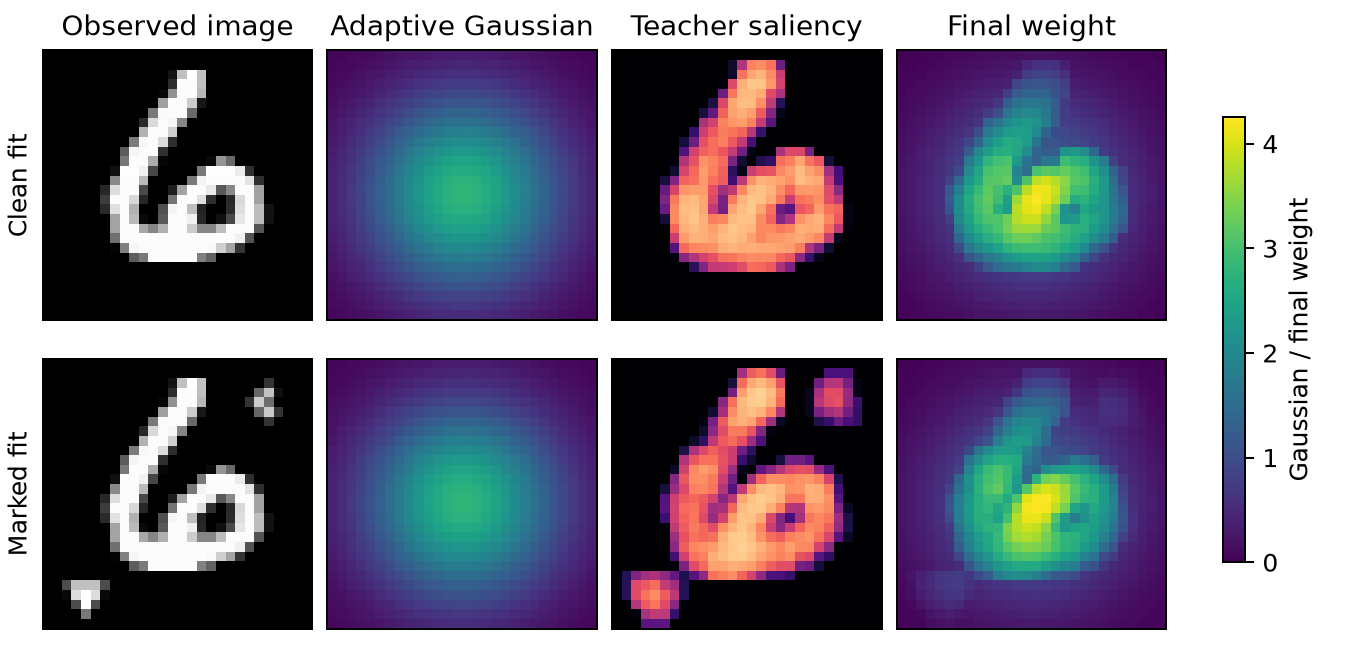
\includegraphics[width=.74\linewidth]{../final/weights.png}\end{center}
\capn{\textbf{Figure 2.} The first training digit in the clean and marked experiments, with each domain's own teacher. Gaussian and final weights share a scale (image mean 1). Saliency runs from dark (0) to bright (1). Only the clean domain fits the teacher and student in the primary experiment.}

\sect{5 \quad Experimental setup}
We sampled 12,000 digits without replacement from MNIST's official training set (split seed 126) and held out the 10,000 official test images. Encoder widths are 784--500--500--2000--10. All student arms use 100 pretraining epochs, 20 K-means restarts for 10 centers, Adam at $10^{-3}$, batch size 256, and 5,600 IDEC updates with target refresh every 140. The teacher uses seed 126. The five paired student seeds are 0--4.

\newpage
\sect{6 \quad Results and analysis}
\textbf{Primary endpoint.} Freeze each clean-trained model and score the same 10,000 digits before and after adding two symbols from 96 combinations of shape, size, angle and brightness. For scoring, the Hungarian algorithm matches clusters to training digit labels once. The marked-fit column uses separate marked training and its own teacher. All ablation arms reconstruct the observed input.

\begin{center}\small\begin{tabular}{lrrr}
\toprule
& \multicolumn{2}{c}{Clean fit} & Marked fit\\
\cmidrule(lr){2-3}Pretraining weights & Clean test & Marked test & Marked test\\\midrule
Ordinary IDEC & 73.23 & 64.62 & 65.14\\
Fixed Gaussian & 74.07 & 68.92 & 68.80\\
Saliency only & 71.83 & 64.33 & 67.51\\
Adaptive Gaussian & 76.20 & 70.28 & 69.71\\
Fixed Gaussian $\times$ saliency & 75.95 & 71.51 & 70.52\\
Adaptive $\times$ shuffled saliency & 73.80 & 68.47 & 68.63\\
\midrule
\textbf{Adaptive $\times$ aligned saliency} & \textbf{76.10} & \textbf{71.59} & \textbf{71.06}\\
\bottomrule
\end{tabular}
\end{center}
\capn{\textbf{Table 3.} Mean held-out digit accuracy (\%) over five paired seeds. The middle numeric column is the primary endpoint. Aligned saliency uses the input's own map. Shuffling substitutes another training image's map while preserving the input's adaptive center.}

Ordinary IDEC lost 8.62 points when marks appeared at test time, compared with 4.50 for the final model. The latter also gained 2.86 points on clean digits. It gained $6.98\pm5.19$ points over ordinary IDEC and $2.67\pm2.01$ over the fixed Gaussian on the primary endpoint, both positive in every seed. With marked training and testing its ACC rose from 65.14\% to 71.06\%. Its redraw flip rate fell from 2.99\% to 2.47\%.

\begin{center}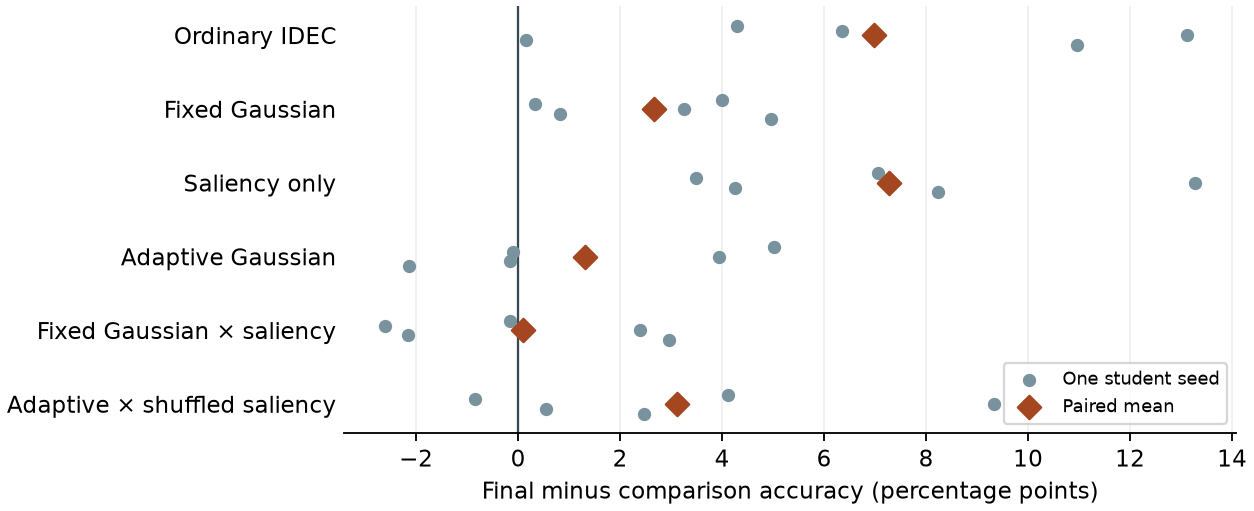
\includegraphics[width=.80\linewidth]{../final/paired.png}\end{center}
\capn{\textbf{Figure 3.} Final minus comparison accuracy on marked test digits after clean training. Each dot is a difference for one matched seed. Positive values favor the final model. Diamonds show means.}

\textbf{Which component helped?} Saliency alone scored 64.33\%, close to ordinary IDEC. With an adaptive Gaussian, the input's own saliency gained 3.12 points over shuffled saliency (four of five seeds), supporting a role for image alignment. Adding saliency to the adaptive Gaussian gained 1.31 points (two of five positive). Moving the center with aligned saliency gained just 0.09 points (paired SD 2.54, two of five positive). The interaction, the saliency gain with an adaptive center minus the gain with a fixed center, was $-1.28\pm3.09$ points. The results leave the additional value of adapting a saliency-weighted center unresolved.

\newpage
\sect{6.1 \quad What does the frozen encoder retain?}
Higher digit accuracy alone leaves open what happens to background information inside the ten-dimensional code. We changed only the brightness of two detached symbols. Their locations, shapes, sizes and angles stayed fixed, and every digit supplied both a dim and a bright view. The brightness label therefore carries no information about digit identity.

\begin{center}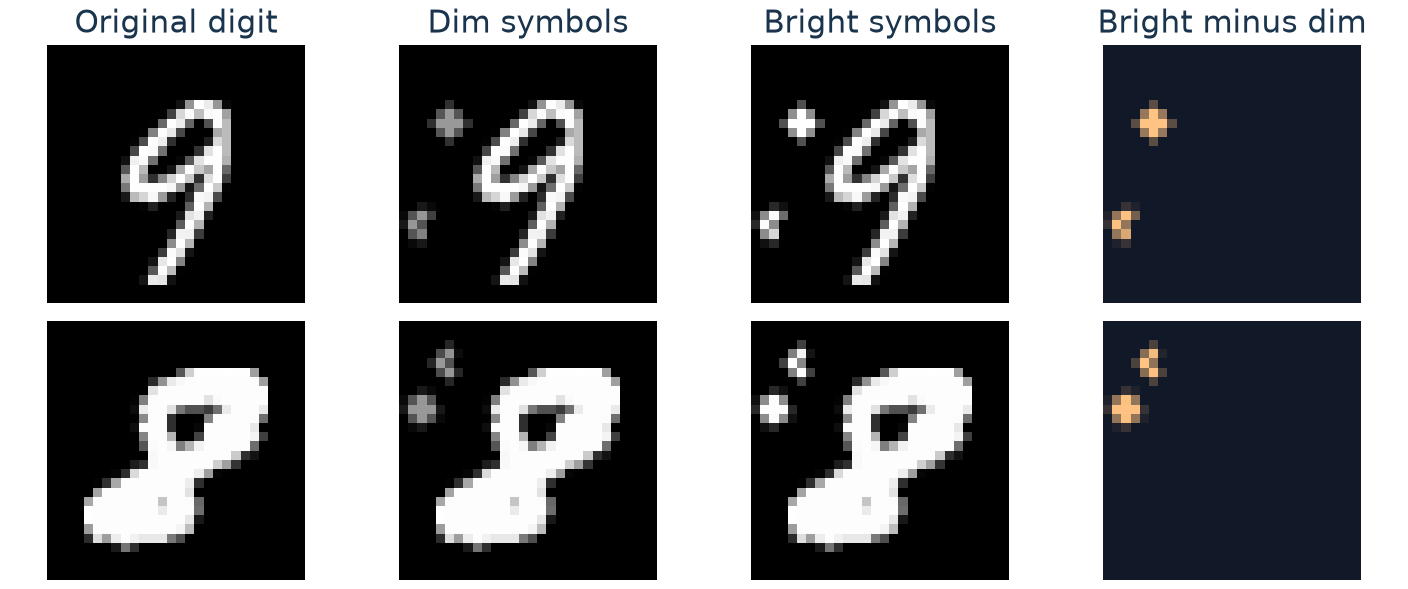
\includegraphics[width=.75\linewidth]{../background_probe/pairs.png}\end{center}
\capn{\textbf{Figure 4.} The first two held-out pairs. Subtracting the dim image from the bright image leaves only the two symbols. Brightness levels 0.6 and 1.0 come from the original background generator.}

We froze ordinary and weighted students after IDEC fine-tuning. For each student we fitted a linear readout on 4,000 independent digits and tested it on 4,000 more. The paired readout learns a direction in code space and decides which member of a new pair contains the brighter symbols. A separate single-image readout sees just one code. Both have a 50\% chance level. The marked-training comparison tests encoders that actually saw symbols during reconstruction training.

\begin{center}\small\setlength{\tabcolsep}{5pt}\begin{tabular}{llrrrrr}\toprule
& & \multicolumn{2}{c}{Brightness ACC} & Code & Cluster & Digit\\
\cmidrule(lr){3-4}Training & Student & Paired & Single & distance & flips & ACC\\\midrule
Marked & Ordinary & 91.93 & 53.02 & 0.254 & 4.16 & 64.12\\
Marked & Adaptive & 93.35 & 53.34 & 0.253 & 3.19 & 70.54\\
Clean & Ordinary & 92.95 & 55.68 & 0.450 & 11.32 & 62.87\\
Clean & Adaptive & 91.36 & 55.42 & 0.438 & 7.60 & 70.43\\
\bottomrule\end{tabular}
\end{center}
\capn{\textbf{Table 4.} Means across five paired seeds. Brightness and digit ACC and cluster flips are percentages. Digit ACC averages the two marked views. Code distance is the mean distance between a digit's dim and bright codes after whitening by the clean calibration covariance.}

\textbf{Primary result.} After marked training, the readout identified the brighter view in 91.93\% of pairs with ordinary IDEC and 93.35\% with our model. The paired increase was $1.42\pm1.70$ points (four of five seeds). On a single image the readouts scored only 53.02\% and 53.34\%. The background difference remains linearly accessible when the readout can compare two versions of the same handwriting.

Brightening the symbols switched the assigned cluster on 4.16\% of digits with ordinary IDEC and 3.19\% with our method. The switch rate fell in every seed. Mean digit ACC on these marked views rose from 64.12\% to 70.54\%. A code can register the change in background while its nearest cluster center stays the same.

After \emph{clean-only} training, paired brightness accuracy fell from 92.95\% to 91.36\% and cluster flips fell from 11.32\% to 7.60\%, both in every seed. Thus the readout effect depends on training exposure, while the direction of the cluster-stability effect agrees across the two training domains. Randomly exchanging brightness labels within test pairs gave about 50\% in each condition.

\newpage
\sect{7 \quad Limitations and conclusion}
\textbf{What receives weight?} We used the generator's clean and marked training images after fitting to audit the weights. Ordinary IDEC assigns weight 1 to every pixel. In the marked-training branch, the final method assigns a mean of 2.62 to digit ink and 0.91 to symbol pixels. The fixed Gaussian alone gives 1.78 and 0.66. Saliency can emphasize visible symbols as well as ink. The final method increases the relative emphasis on handwriting compared with uniform loss, even though the simpler Gaussian assigns a smaller absolute weight to symbols.

\textbf{What does the evidence establish?} The clean-target intervention shows that the reward for reproducing known background can cost digit accuracy even when every input is held fixed. The brightness readouts measure one attribute of the final code. They cannot establish how much of the digit accuracy gain that attribute explains. The improvement on clean digits also leaves room for a change in the representation of handwriting itself.

\textbf{Does a more flexible Gaussian help?} In the clean fitting set the estimated center lies only 0.67 pixels from the midpoint on average, compared with a width of seven. On a second 10,000-digit marked holdout ordinary IDEC reached 64.65\%, the adaptive circle reached 70.65\%, and an ellipse elongated along the image's main intensity axis reached 70.98\%. The ellipse improved on the circle in three of five seeds, below our four-seed selection threshold. The circular window remains our final choice. Central distractors and natural photographs remain open questions. The five student seeds share one teacher and one split per domain.

\textbf{Comparison with DEC.} Clean-trained DEC reached 75.62\% on the original marked test, above the final IDEC variant's 71.59\% in every seed. DEC still uses reconstruction for initialization and then updates its encoder using only its clustering objective.

\textbf{Conclusion.} Uniform reconstruction can reward information that impairs digit clustering. On the original clean-trained marked test our adaptive circular Gaussian with aligned saliency gains 6.98 points over ordinary IDEC. A fixed center captures nearly all of that gain. When only a background attribute changes, the adaptive model can encode the change and still make a more stable clustering decision.

\sect{8 \quad References and reproducibility}
{\small
[1] X. Guo, L. Gao, X. Liu and J. Yin. \emph{Improved Deep Embedded Clustering with Local Structure Preservation}. IJCAI, 2017. \href{https://www.ijcai.org/proceedings/2017/243}{Proceedings and paper.}\par
[2] J. Xie, R. Girshick and A. Farhadi. \emph{Unsupervised Deep Embedding for Clustering Analysis}. ICML, 2016. \href{https://proceedings.mlr.press/v48/xieb16.html}{Proceedings and paper.}\par
[3] X. Guo. \href{https://github.com/XifengGuo/IDEC/tree/4a661c211f082022249758ab3312f7db21e2aa99}{Official IDEC implementation} and \href{https://github.com/XifengGuo/data-and-models/tree/d361bfe06686c0762df58624ef95a8c0fc9162be}{pretrained MNIST weights}. Y. LeCun, C. Cortes and C. Burges. \href{https://www.tensorflow.org/datasets/catalog/mnist}{MNIST handwritten digits.}\par
\textbf{Project materials.} Our PyTorch implementation, fitting commands, per-image assignments, probe embeddings and paired comparisons are in the \href{https://github.com/JohnR31N/cs126FinalProj/tree/idec-final-v2.2}{versioned public repository}. An independent seed-0 refit from raw MNIST scored 72.86\% on marked digits, compared with 73.07\% in the archived seed-0 run. The five-seed means use the original runs.}
\end{document}
